%%%%%%%% Method::tauRF
\clearpage
\begin{figure}[htbp]
  \begin{center}
      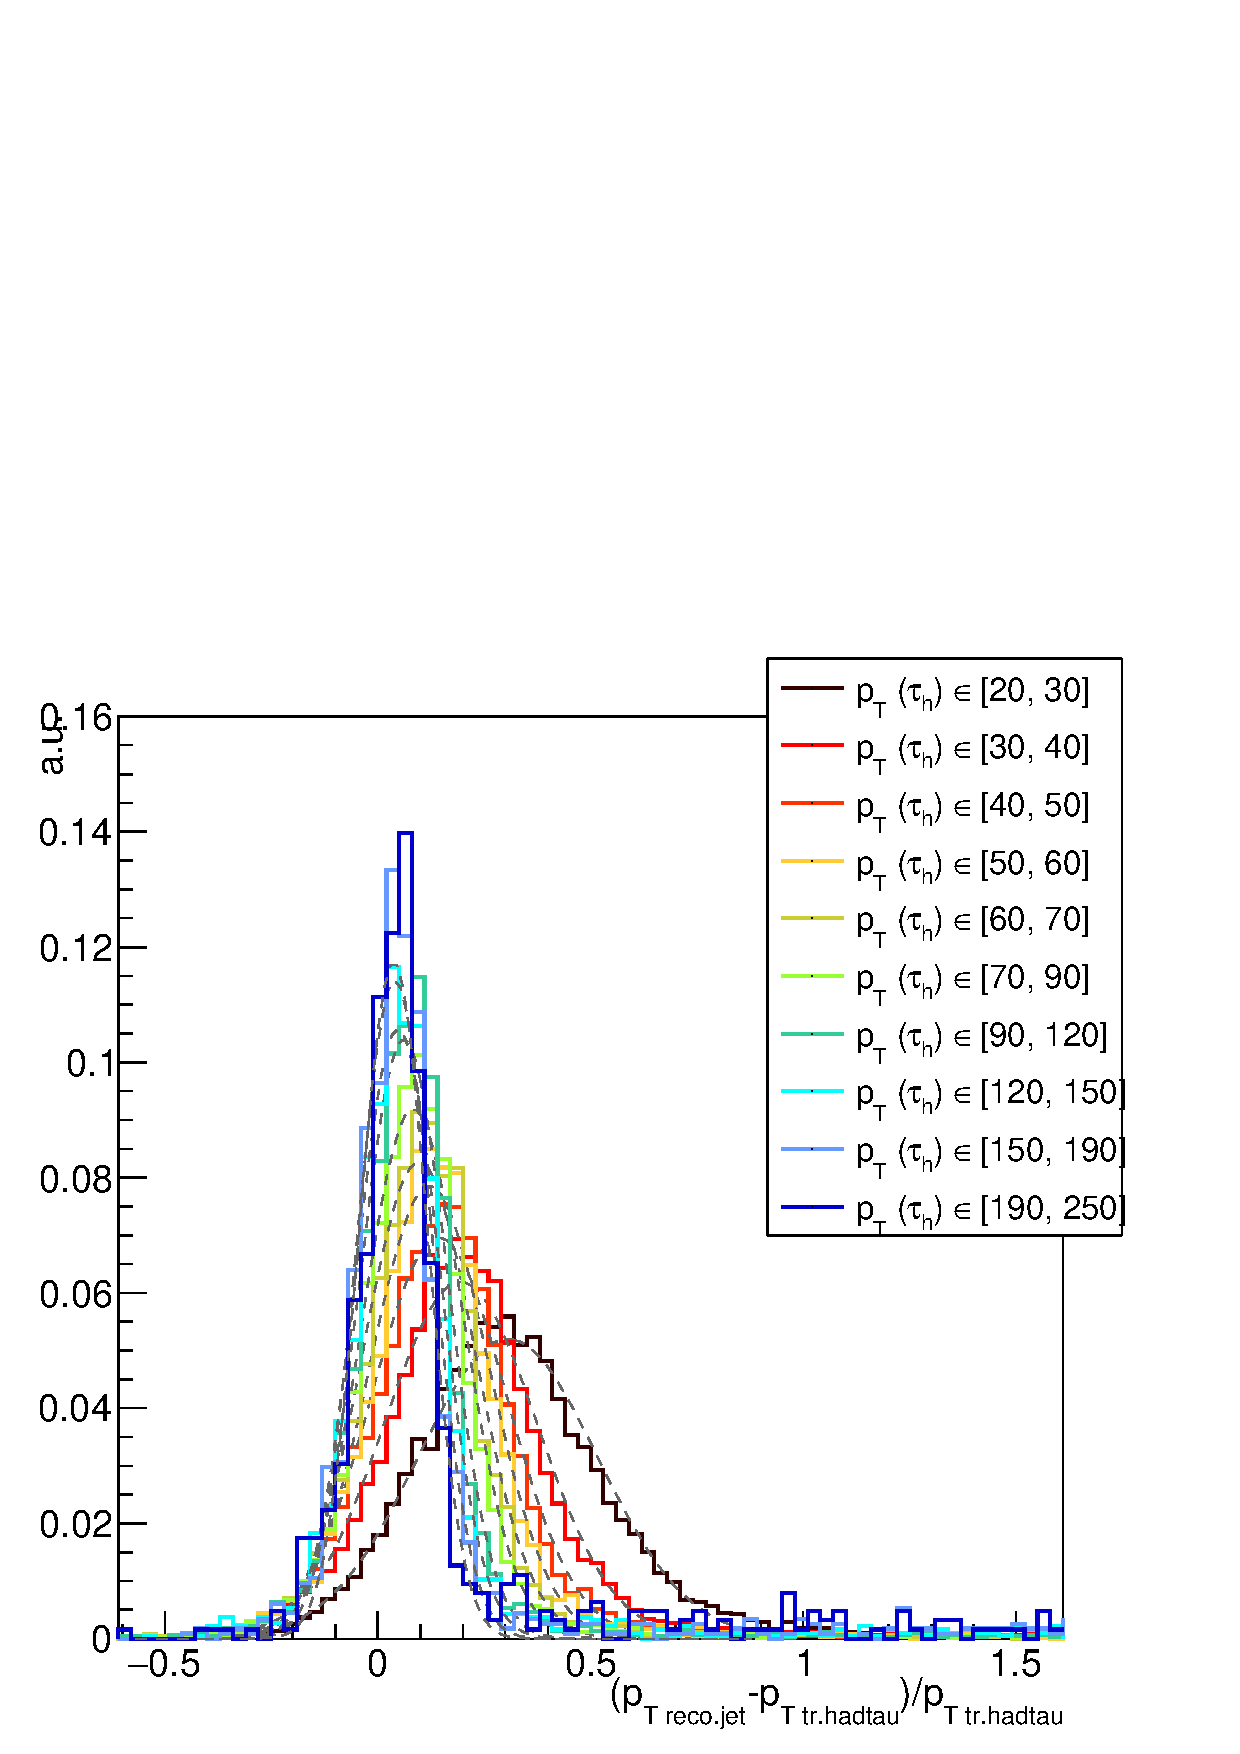
\includegraphics[width=100mm]{figures/BGestimation/ObjReplacement/method/tauRF/ptResidual.pdf} 
      \caption{}
      \label{fig::ObjReaplce::tau_ptResidual}
    %
    \begin{minipage}[t]{.45\textwidth}
      \centering        
      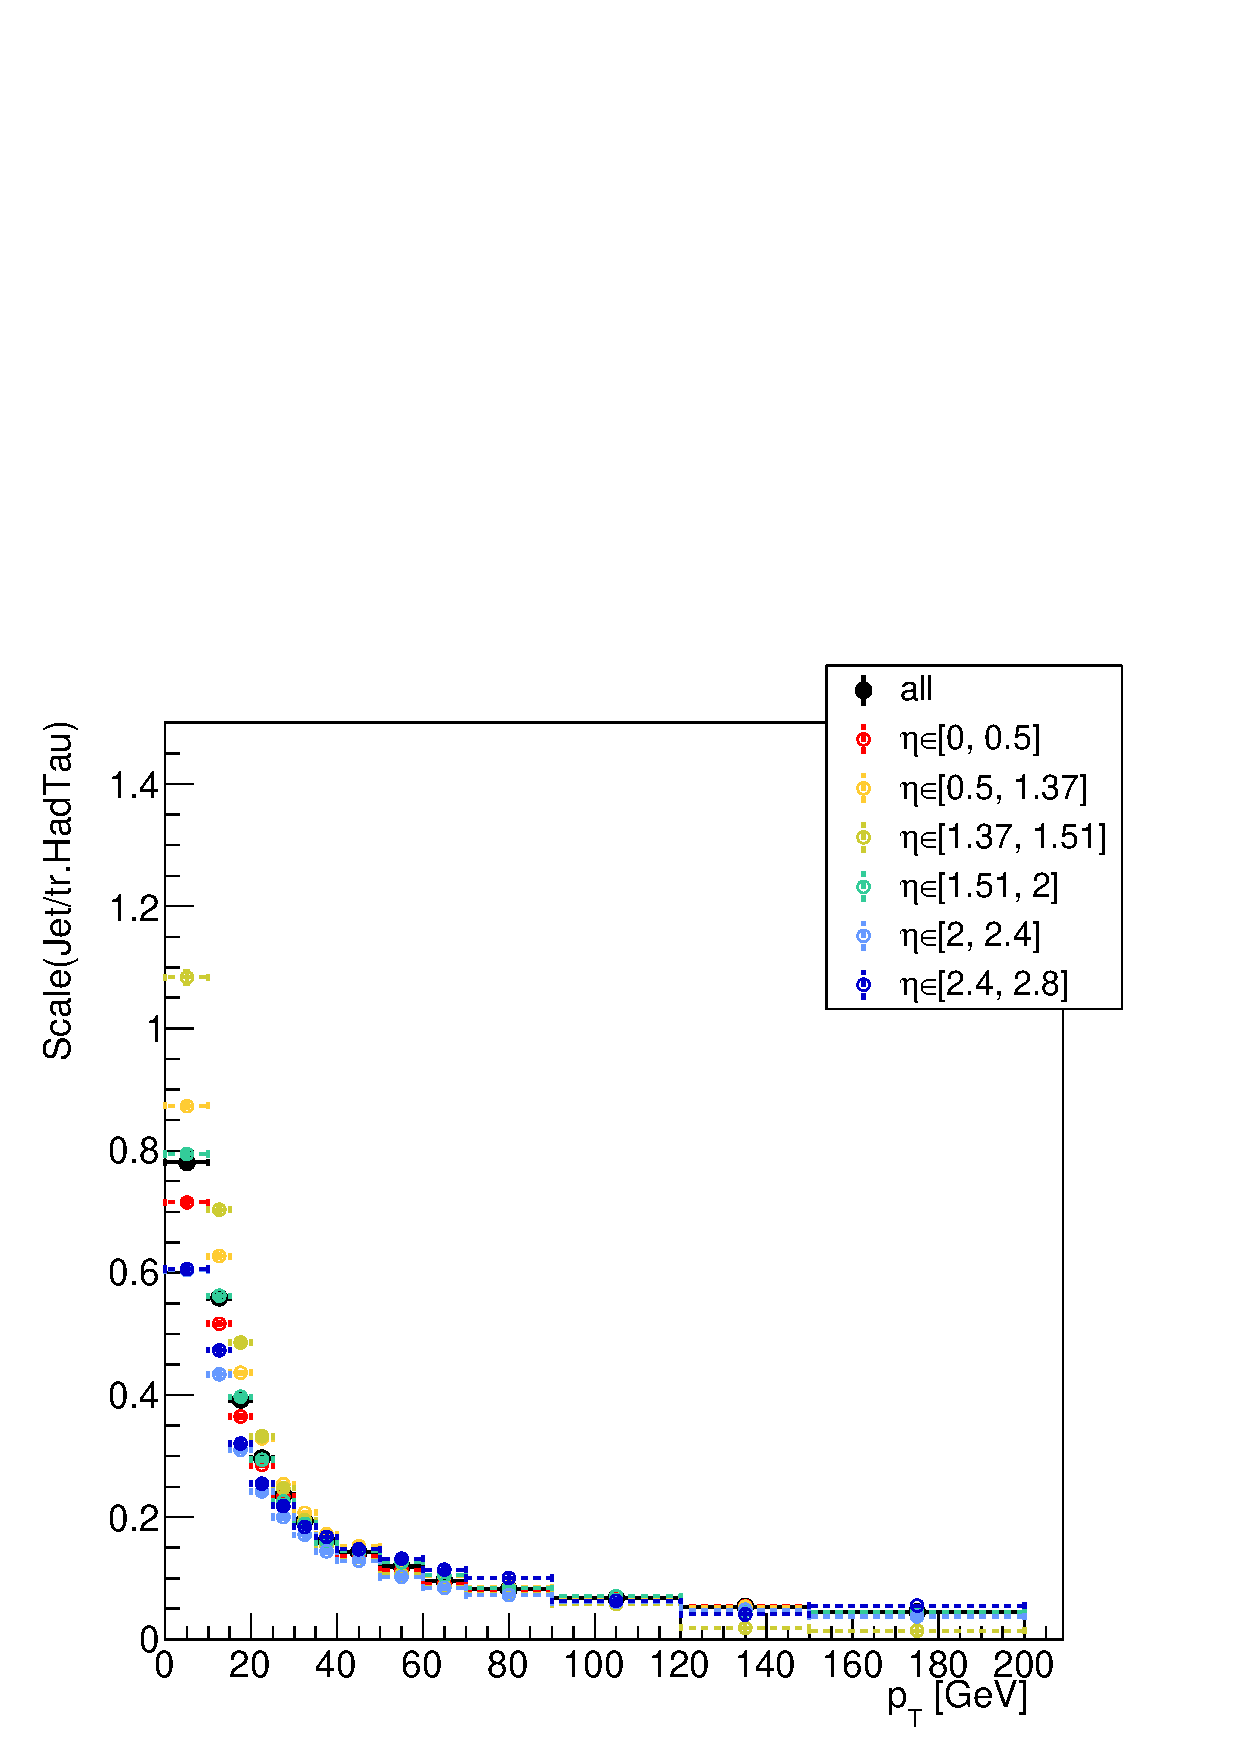
\includegraphics[width=85mm]{figures/BGestimation/ObjReplacement/method/tauRF/tauJet_scale.pdf} 
      \caption{Scale of anti-Kt4 jets for truth hadronic taus, defined as the mean of reco. $p_T(\tau_{h})$/truth $p_T(\tau_{h})-1$ distribution. Truth $p_T(\tau_{h})$ is defined as the transverse component of $|\bm{p}(\tau)-\bm{p}(\nu_{tau})|$ while the reconstructed one is defined as the $p_T$ of an anti-Kt4 jet $\Delta R$-matched to it.}
      \label{fig::ObjReaplce::tau_scale}
    \end{minipage}
    \hfill
    \begin{minipage}[t]{.45\textwidth}
      \centering
      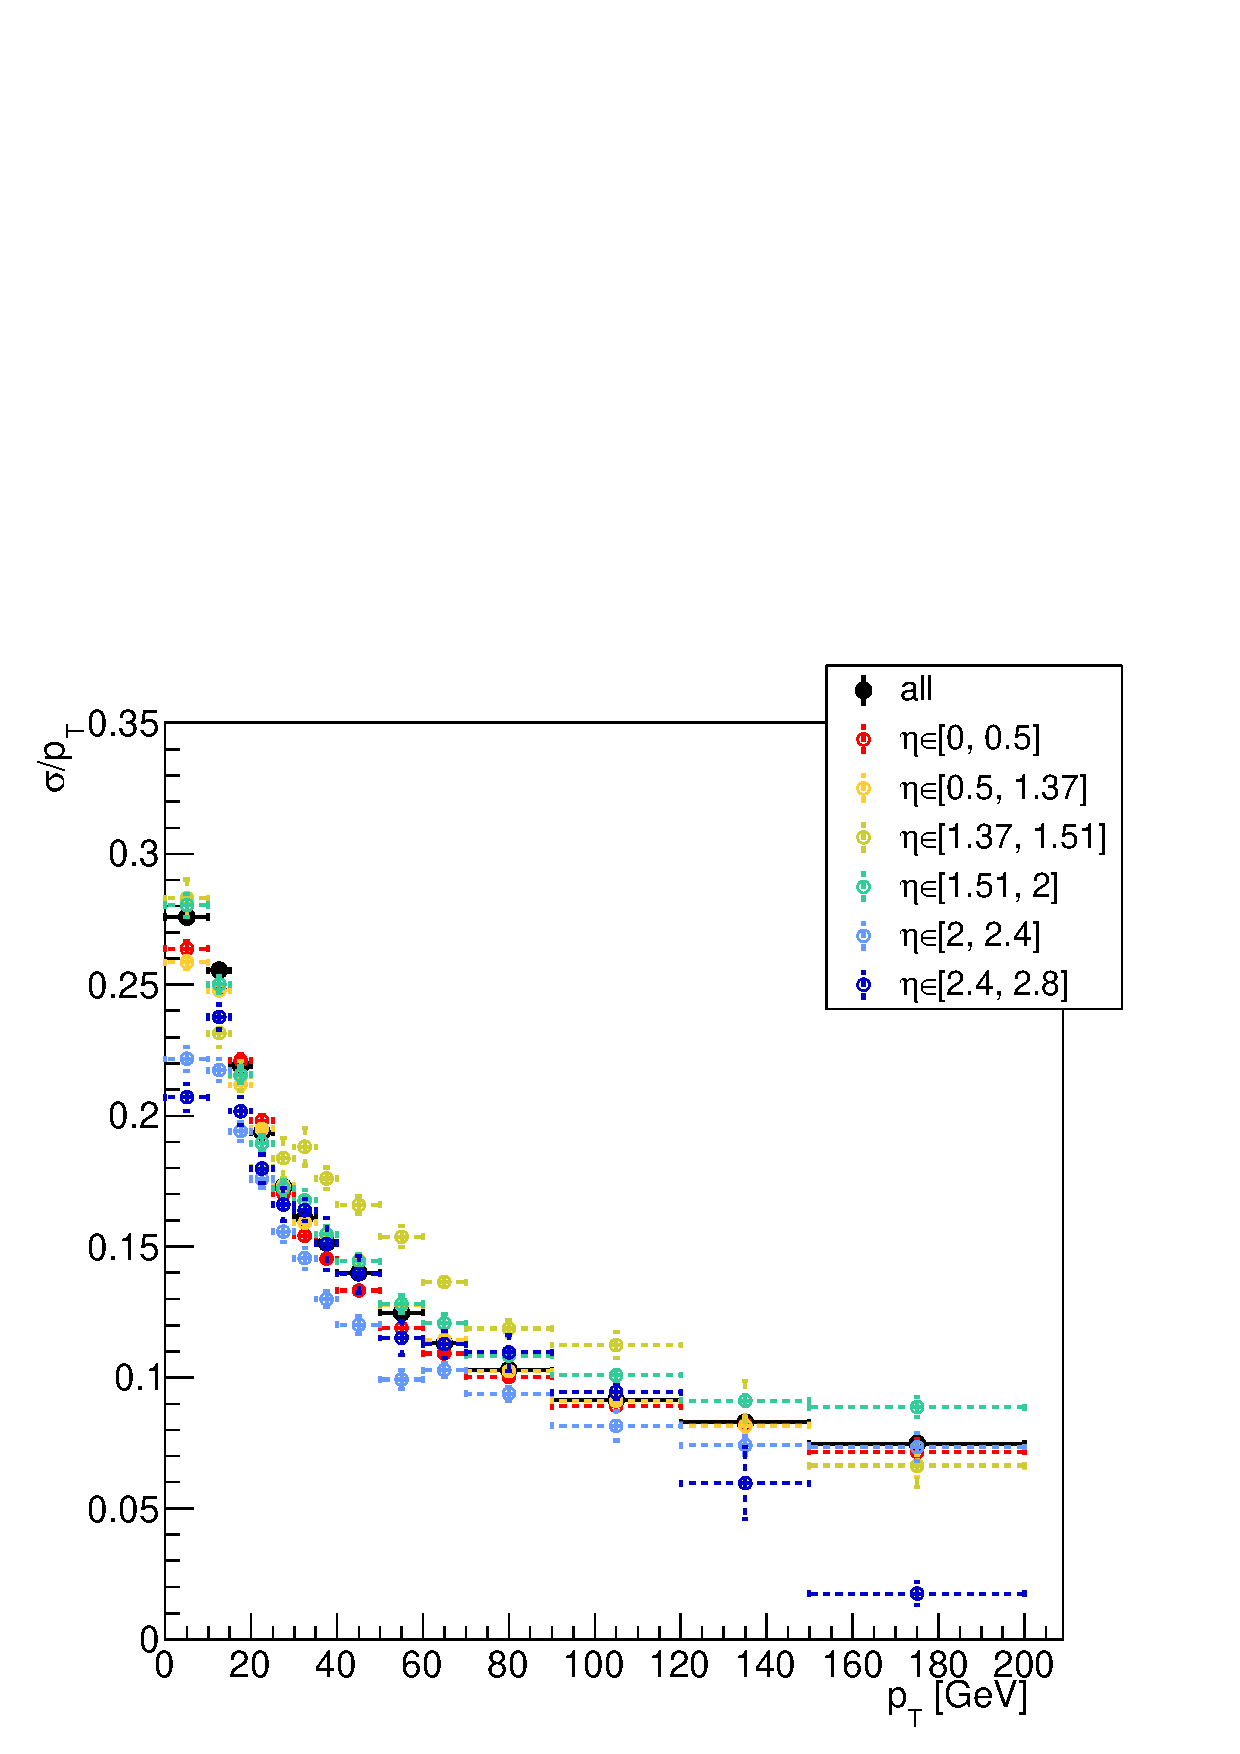
\includegraphics[width=85mm]{figures/BGestimation/ObjReplacement/method/tauRF/tauJet_resol.pdf}
      \caption{Resolution of hadronic tau, defined as the gaussian-fitted RMS of reco. $p_T(\tau_{h})$/truth $p_T(\tau_{h})-1$ distribution. Reco. $p_T(\tau_{h})$ is defined as the $p_T$ of $\Delta R$-matched anti-Kt4 jet.}
      \label{fig::ObjReaplce::tau_resol}
    \end{minipage}
    %              
  \end{center}  
\end{figure}
\clearpage
\begin{figure}[htbp]
  \begin{center}
    \begin{minipage}[t]{.45\textwidth}
      \centering
      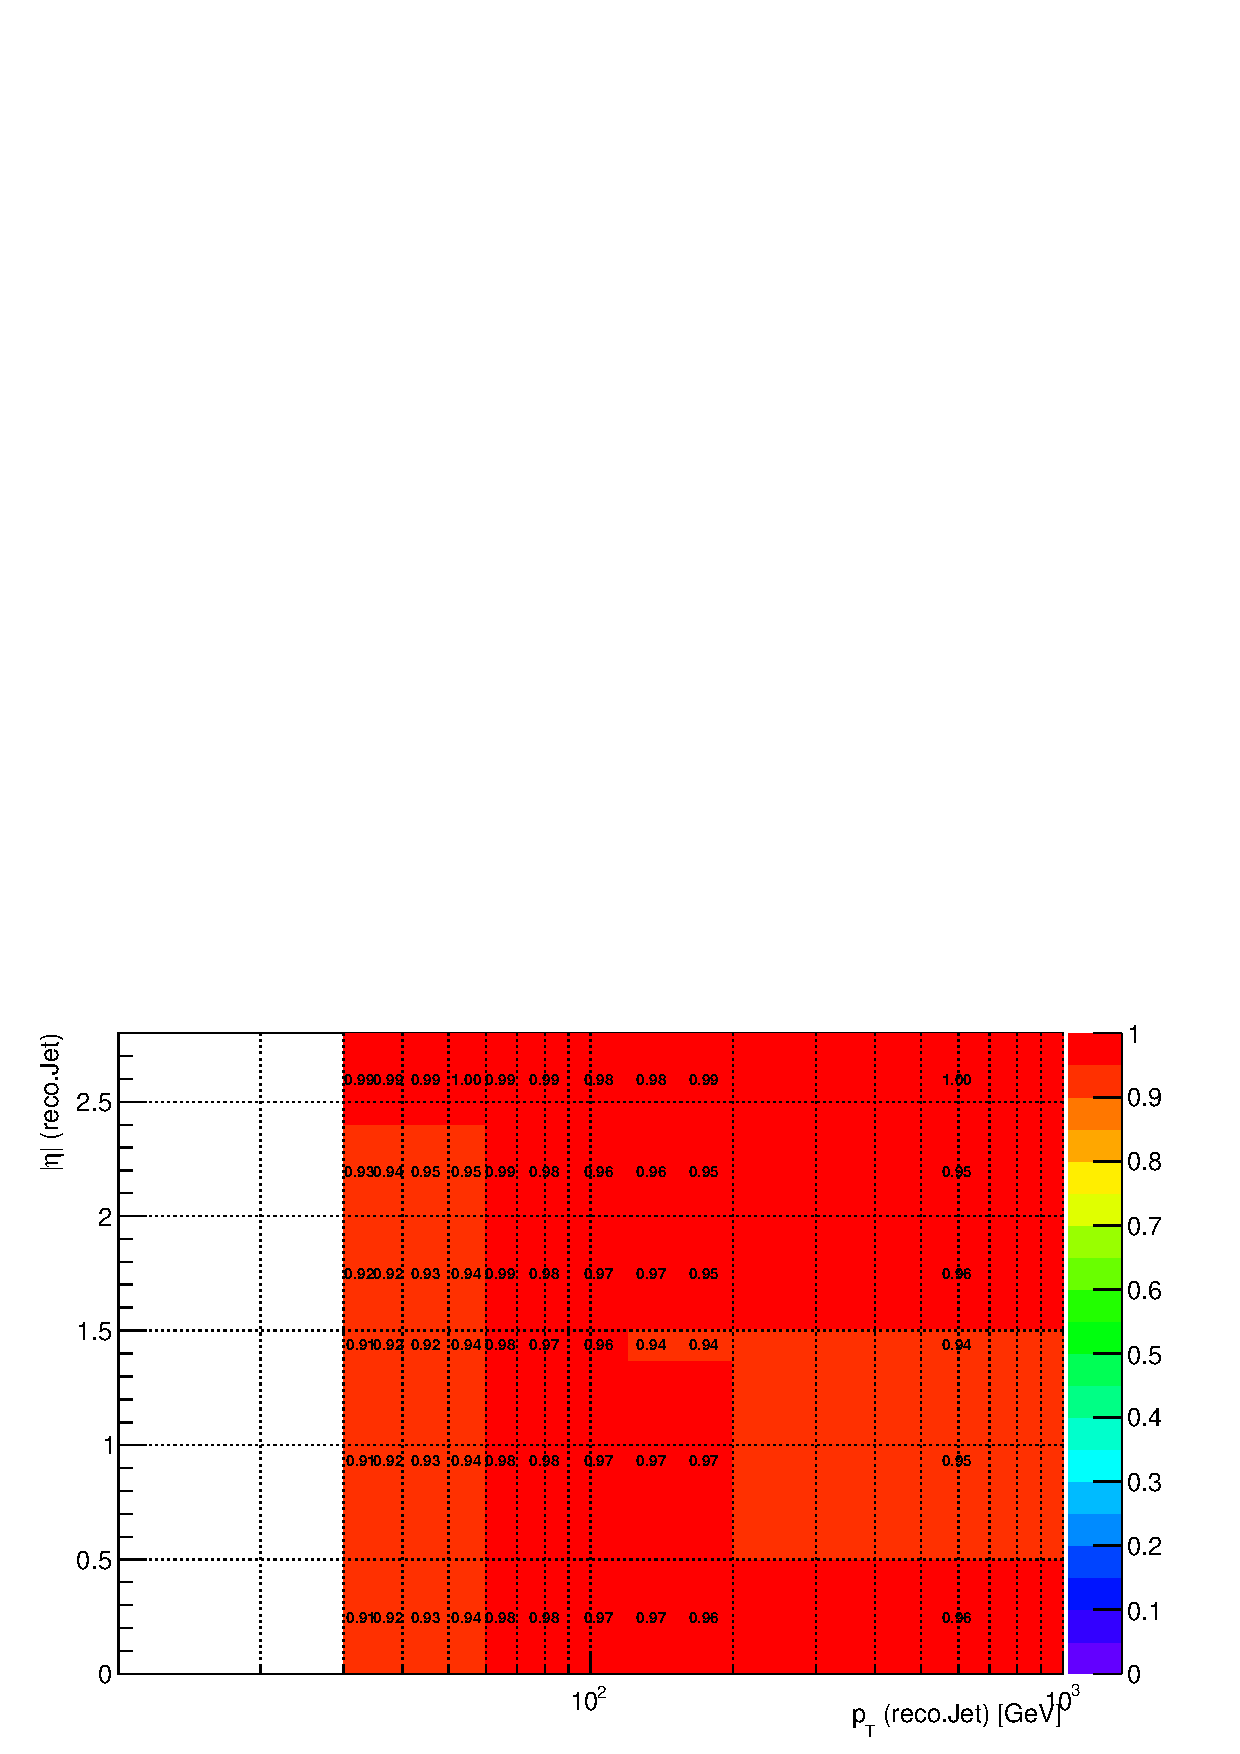
\includegraphics[width=85mm]{figures/BGestimation/ObjReplacement/method/tauRF/heff_vs_recoJetPt_recoJetEta.pdf}
      \caption{Fraction of signal jet candidates that pass the signal jet requirement, parametrized as function of $p_{\mathrm{T}}$ and $\eta$ of reconstructed jets.}
      \label{fig::ObjReaplce::effJVT}
    \end{minipage}
    \hfill
    \begin{minipage}[t]{.45\textwidth}
      \centering
      \includegraphics[width=75mm]{figures/BGestimation/ObjReplacement/method/tauRF/hadTau_bTagScore.pdf}
      \caption{Profile of b-tagging score (MV2c10) for tau jets, calculated from ttbar MC.}
      \label{fig::ObjReaplce::tau_bTagScore}
    \end{minipage}
    %
  \end{center}
\end{figure}
%%%%% Method::effMap 
%\clearpage
\begin{figure}[htbp]
  \begin{center}
    %
    \begin{minipage}[t]{.45\textwidth}
      \centering
      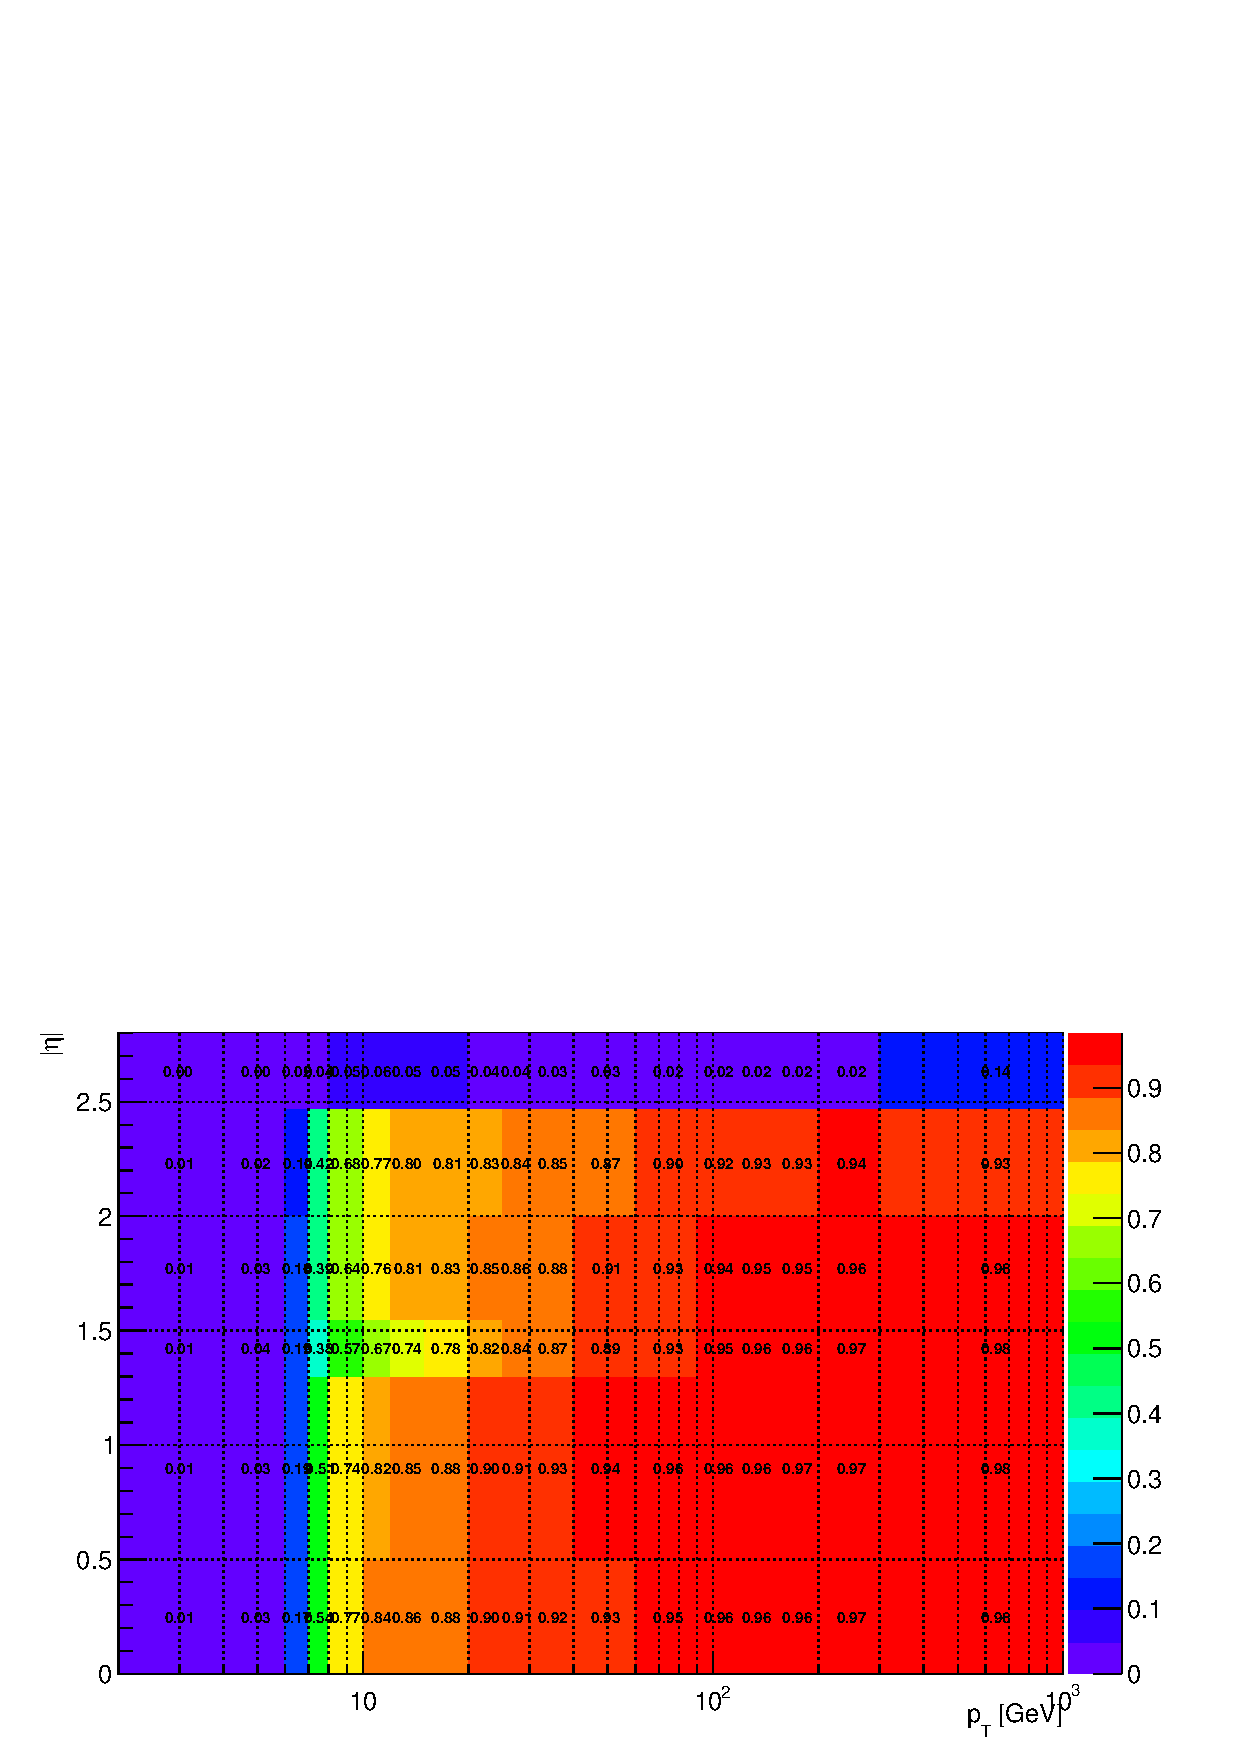
\includegraphics[width=75mm]{figures/BGestimation/ObjReplacement/method/lepeff/el_trPtEta_truthToID.pdf}
      \hspace{10mm} (a)
      \label{fig::ObjReaplce::heff_mc_el_truthToID}
    \end{minipage}
    \begin{minipage}[t]{.45\textwidth}
      \centering
      \includegraphics[width=75mm]{figures/BGestimation/ObjReplacement/method/lepeff/el_trPtEta_truthToSig.pdf}
      \hspace{10mm} (b)
      \label{fig::ObjReaplce::heff_mc_el_truthToSig}
    \end{minipage}
    %
    \begin{minipage}[t]{.45\textwidth}
      \centering
      \includegraphics[width=75mm]{figures/BGestimation/ObjReplacement/method/lepeff/mu_trPtEta_truthToID.pdf}
      \hspace{10mm} (c)
      \label{fig::ObjReaplce::heff_mc_mu_truthToID}
    \end{minipage}
    \begin{minipage}[t]{.45\textwidth}
      \centering
      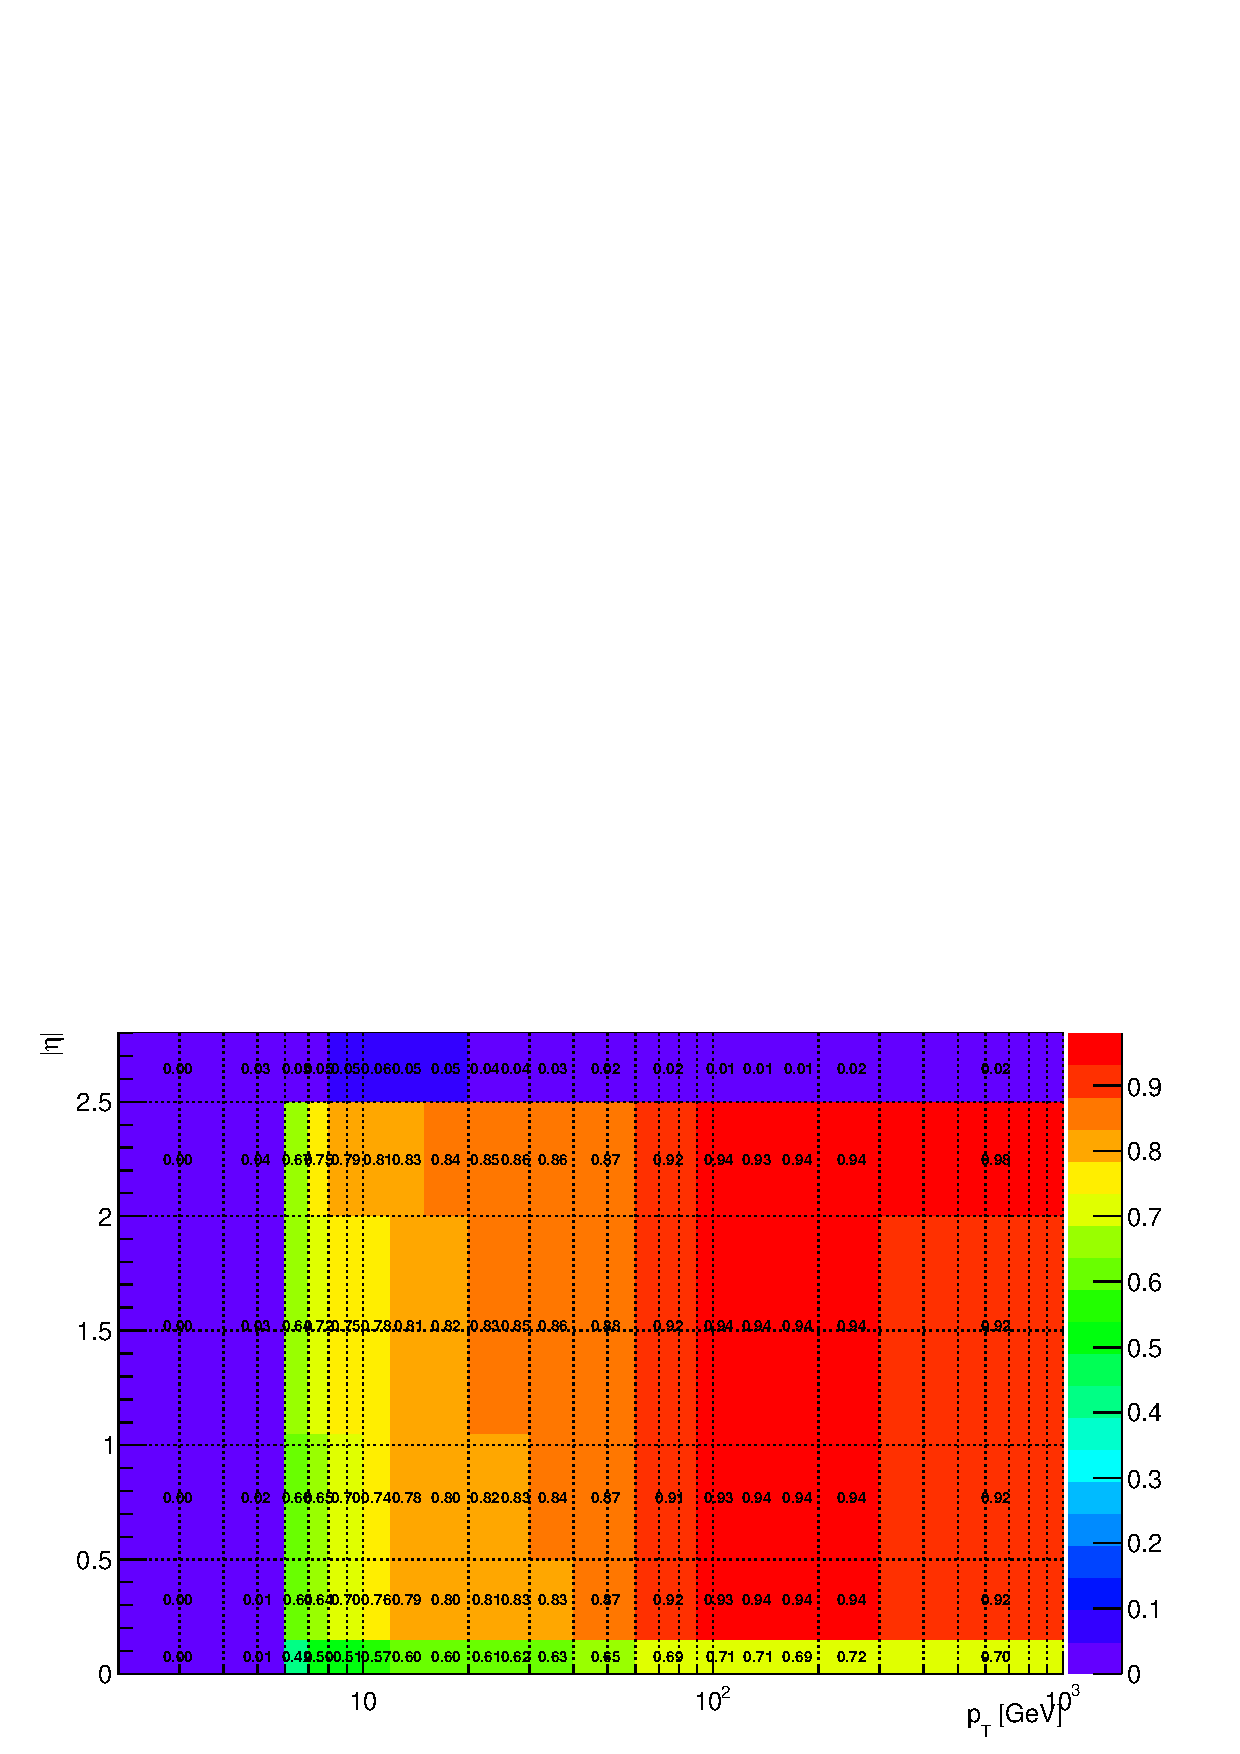
\includegraphics[width=75mm]{figures/BGestimation/ObjReplacement/method/lepeff/mu_trPtEta_truthToSig.pdf}
      \hspace{10mm} (d)
      \label{fig::ObjReaplce::heff_mc_mu_truthToSig}
    \end{minipage}
    %
    \caption{Off-line selection efficiency used in transfer factor calulation. (a) Efficiency of electrons passing reconstruction and ID. (b) Efficiency of electrons passing signal lepton requirement.  (c) Efficiency of muons passing reconstruction and ID. (d) Efficiency of muons passing signal lepton requirement.}
    \label{fig::ObjReaplce::lep_efficiency}
  \end{center}
\end{figure}
